\documentclass[11pt]{article}
\usepackage{sectsty}
\usepackage{graphicx}
\usepackage{floatrow}
\usepackage{array}
\usepackage{biblatex}
\addbibresource{ref.bib}
\addbibresource{drb.bib}
\addbibresource{syc.bib}

% Margins
\topmargin=-0.45in
\evensidemargin=0in
\oddsidemargin=0in
\textwidth=6.5in
\textheight=9.0in
\headsep=0.25in

\title{CS6000 - Introduction to Research (Week 1 Journal)}
\author{ Ken Lew }
\date{\today}

\begin{document}
\maketitle

\section{Section 1}

From Week 1, the definition of research is “a combination of investigation.” I hope to learn everything that I can about “investigation” and common tools in accomplishing that. I believe one of my skills, like reading research papers more effectively, can be further improved. More importantly, I bring in the mentality of being curious and grit. Being curious allows me to explore and wonder while grit allows me to dig deep into certain topics that would help with my research. My mission and goal for this CS6000 course is to get the perspective in understanding elements of good research that sparks my interest and passion, while making an impact on society. I am currently in my first semester of the PhD security program here at University of Colorado, Colorado Springs. With the nature of the program, I would also like to learn on how to effectively present my ideas and convey my research to the languages of different audiences. My research topic will be close to Blockchain technology with its performances and implementation. 

\begin{center}
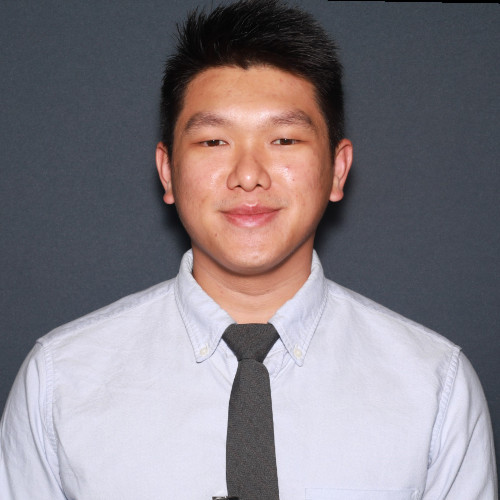
\includegraphics[scale=0.45]{kl.png}
\end{center}

Some of my recent interests besides information technology would be aviation and endurance sports. I have a little more than 100 hours in a Cessna 172M model and I will be running a 50k trail run this coming October.

\section{Section 2}

\subsection{Google Scholar Search}
There are a few steps in Google Scholar Search that I would be able to use in order to be efficient. Here are some main steps:

\begin{enumerate}
  \item Once on the website \texttt{(https://scholar.google.com/)}, I would then look for the 3 line menu bar and navigate to "Advanced Search"
  \item I would then enter my search keywords accordingly into the search criteria. 
  \item After keywords, I can include the author and/or date range that it was published.
\end{enumerate}

\begin{center}
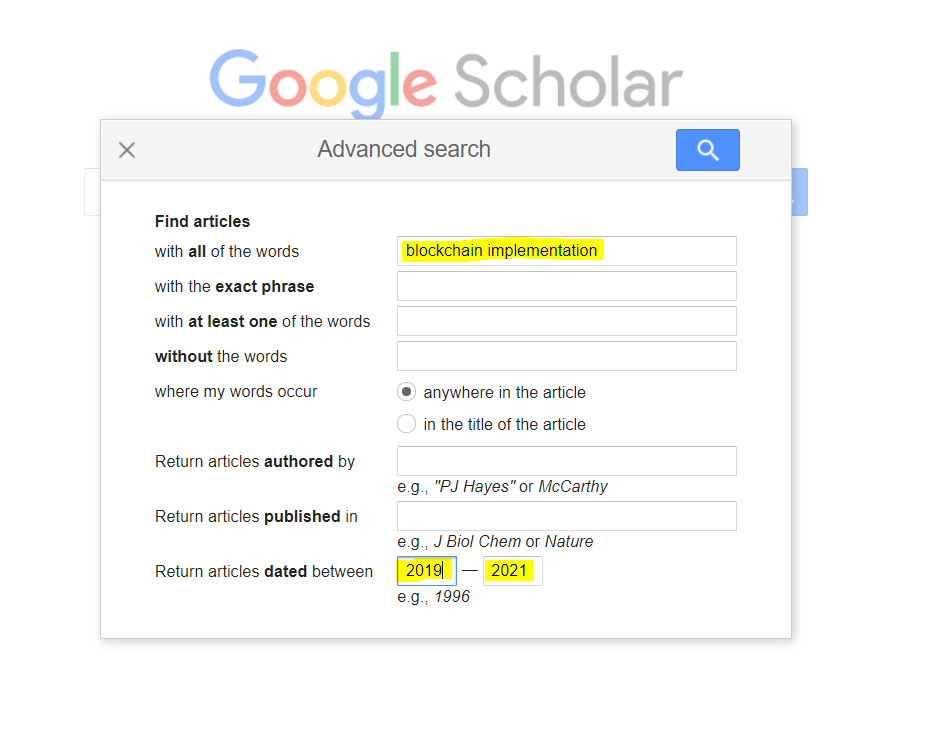
\includegraphics[scale=0.50]{research1.png}
\end{center}


\subsection{Github} 
The \emph{Latex} body of this document is in this Github link here.

\subsection{Lesson Learned}
I have previously used \emph{Overleaf} and \emph{Zotero} for my research papers and projects, as well as Google Scholar. However, I do believe the more I worked on it, the more proficient/efficient I would get in drafting research papers in different format and requirements. Some of my challenges that I have faced this week would include figuring out the citation formatting but soon got clarification from Dr. Boult in completing Section 3.

One lesson I have learned that would have made a difference in my time doing my survey study through research paper is to save and label papers through \emph{Google Scholar} "My Library." This way, it helps me further organize all my thoughts into section/label and would be able to find them whenever I needed to.

In a way, I can now use both \emph{Google Scholar} and \emph{Zotero} to organize my papers and citations. Whereas previously I am only using \emph{Zotero} to do the organizing task. On the side note, using a \emph{Zotero} chrome plug-in help save me time to saving those research paper and citation without much hassle.

\begin{center}
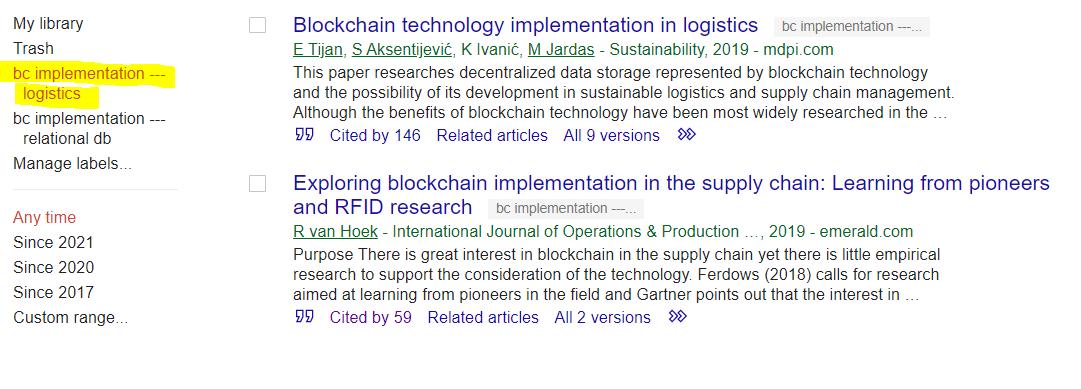
\includegraphics[scale=0.65]{research6.png}
\end{center}

\section{Section 3}

\subsection{Research Papers}
Some of my research papers I have read that is close to being a survey of blockchain application would be as follows: 

\begin{enumerate}
  \item \textbf{Blockchain: How shipping industry is dealing with the ultimate technological leap} speaks about the technological gap that the author have observed the challenges in shipping industry while pointing out the potential of blockchain implementation in the industry as it has already been introduced in maritime sector. \cite{bavassano_blockchain__nodate}
 
  \item \textbf{Blockchain for Supply Chain Traceability: Business Requirements and Critical Success Factors} highlights different perspective on blockchain implementation that includes current implementation practices, the needs of various stakeholders, critical success factors for implementation in order to give an overview of the practicality of the implementation of supply chain traceability. \cite{hastig_blockchain_2020}
  
  \item \textbf{Supply network design to address United Nations Sustainable Development Goals: A case study of blockchain implementation in Thai fish industry} brings a broad overview of the impact of the blockchain implementation in making the fishery industry more sustainable by introducing live tracking and reduces illegal fishing activities. \cite{naoum_supply_nodate}
  
  \item \textbf{Barriers to implementation of blockchain into supply chain management using an integrated multi-criteria decision-making method: a numerical example} recognizes the importance of visibility within the supply chain process and hence focus more on the integration, cost, and implementation. \cite{ozturk_barriers_2020}
  
  \item \textbf{Factors Affecting Implementation of Blockchain in Retail Market in Malaysia} gives a different perspective from the logistics, maritime and implementation. However, the similarities for most of these papers that I have read, highlight the challenges of implementation. \cite{dwyer_expanding_2007} 
  
\end{enumerate}

Here are more related papers that I have found:

\begin{center}
\begin{tabular}{ | m{.5cm} | m{10cm}| m{1cm} | } 
  \hline
  1 & Blockchain applications–usage in different domains & \cite{abou2019blockchain} \\ 
  \hline
  2 & Blockchain security threats, attacks and countermeasures & \cite{siddiqui2020blockchain} \\ 
  \hline
  3 & Blockchain technology: A survey on applications and security privacy challenges  & \cite{mohanta2019blockchain} \\  
  \hline
  4 & A theoretical implementation: Agriculture-food supply chain management using blockchain technology  & \cite{madumidha2019theoretical} \\ 
  \hline
  5 & Implementation of an e-voting scheme using hyperledger fabric permissioned blockchain & \cite{kirillov2019implementation} \\ 
  \hline
  6 & Success factor of implementation blockchain technology in pharmaceutical industry: a literature review & \cite{fernando2019success} \\  \hline
  7 & A correctable public blockchain  & \cite{marsalek2019correctable} \\ 
  \hline
  8 & Study and implementation on the application of blockchain in electronic evidence generation & \cite{chen2020study} \\ 
  \hline
  9 & Modeling the blockchain enabled traceability in agriculture supply chain  & \cite{kamble2020modeling} \\  
  \hline
  10 & Integrating blockchain into supply chain management: A toolkit for practical implementation & \cite{waller2019integrating} \\ 
  \hline
  11 & Towards building a blockchain framework for IoT & \cite{pavithran2020towards} \\ 
  \hline
  12 & Blockchain Technology for Industry 4.0 & \cite{da2020blockchain} \\  
  \hline
  13 & A review of blockchain technology implementation in shipping industry & \cite{jovic2019review} \\ 
  \hline
  14 & A graph model based blockchain implementation for increasing performance and security in decentralized ledger systems & \cite{tsoulias2020graph} \\ 
  \hline
  15 & How will blockchain technology impact auditing and accounting: Permissionless versus permissioned blockchain & \cite{liu2019will} \\  
  \hline
  16 & A permissioned blockchain-based implementation of LMSR prediction markets & \cite{carvalho2020permissioned} \\ 
  \hline
  17 & The application of blockchain technology in the maritime industry & \cite{czachorowski2019application} \\ 
  \hline
  18 & Advanced applications of blockchain technology & \cite{kim2020advanced} \\  
  \hline
  19 & Blockchain Implementation in Hotel Management  & \cite{flecha2020blockchain} \\ 
  \hline
  20 & Permissioned blockchain through the looking glass: Architectural and implementation lessons learned & \cite{gupta2020permissioned} \\  
  \hline
\end{tabular}
\end{center}

\subsection{Math Equation Input}

One of the interesting paper that I have found is regarding 'Digital Investigation.' The author of the paper wanted to develop and test images used by judicial court that is efficient and credible. Hence, for the purpose of testing and analysis, images are processed and encrypted with digital image watermark to become a blockchain-enabled electronic evidence.

\[PSNR = 10 * log_{10} (((2^n-1)^2)/MSE)\]

The equation depicted above is to evaluate the 'Peak Signal to Noise Ratio' (PSNR) where it will give the differences between the original image from the judicial court compared to watermarked image downloaded. \cite{chen2020study}

\subsection{Advisor's Paper Publication (Class Exercise)}

Through the exercise with \emph{Google Scholar}, my approach is to find the author's profile, in which this case would be Dr. Terrance Boult and Dr. Sang-Yoon Chang. From there, I will be selecting the top 5 most "cited by" article on the profile that list all the publication.

\subsubsection{Dr. Terrance E. Boult}

\begin{center}
\begin{tabular}{ | m{.5cm} | m{10cm}| m{1cm} | } 
  \hline
  1 & Toward open set recognition & \cite{scheirer_toward_2013} \\ 
  \hline
  2 & Towards open set deep networks  & \cite{bendale_towards_2016} \\ 
  \hline
  3 & Constraining object features using a polarization reflectance model  & \cite{noauthor_constraining_nodate} \\  
  \hline
  4 & Separation of reflection components using color and polarization  & \cite{nayar_separation_1997} \\ 
  \hline
  5 & Cracking fuzzy vaults and biometric encryption & \cite{scheirer_cracking_2007} \\ 
  \hline
\end{tabular}
\end{center}

\begin{center}
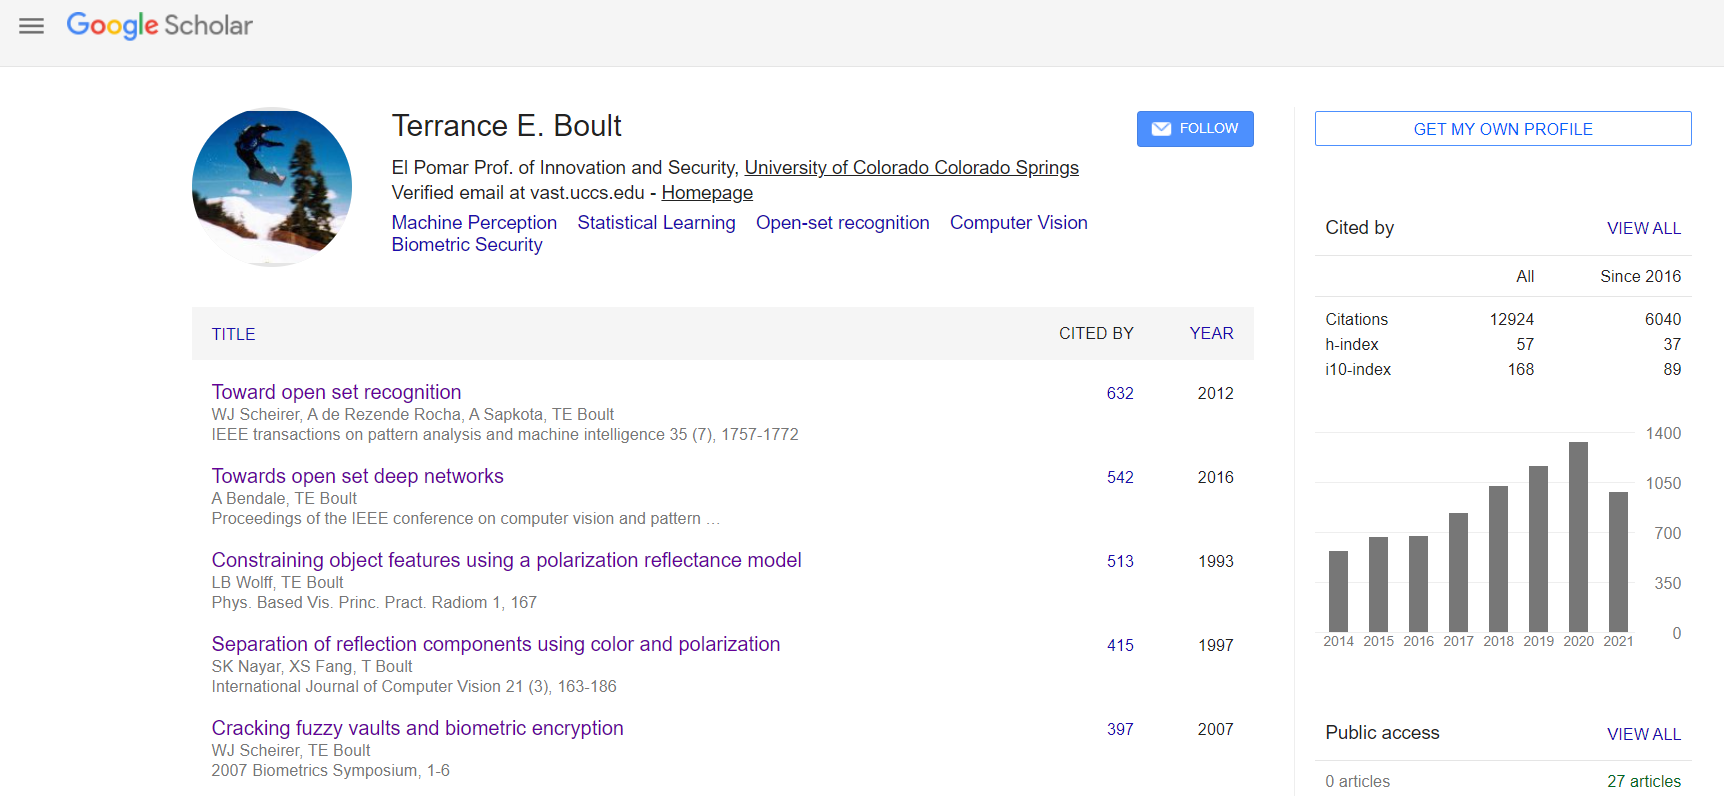
\includegraphics[scale=0.45]{terry1.PNG}
\end{center}

\subsubsection{Dr. Sang-Yoon Chang}

\begin{center}
\begin{tabular}{ | m{.5cm} | m{10cm}| m{1cm} | } 
  \hline
  1 & Body Area Network Security: Robust Key Establishment Using Human Body Channel. & \cite{chang_body_nodate} \\ 
  \hline
  2 & Enabling dynamic access control for controller applications in software-defined networks  & \cite{padekar_enabling_2016} \\ 
  \hline
  3 & Fast IP hopping randomization to secure hop-by-hop access in SDN  & \cite{chang_fast_2019} \\  
  \hline
  4 & SimpleMAC: A jamming-resilient MAC-layer protocol for wireless channel coordination  & \cite{chang_simplemac_2012} \\ 
  \hline
  5 & Uncle-block attack: Blockchain mining threat beyond block withholding for rational and uncooperative miners & \cite{noauthor_uncle-block_nodate} \\ 
  \hline
\end{tabular}
\end{center}

\begin{center}
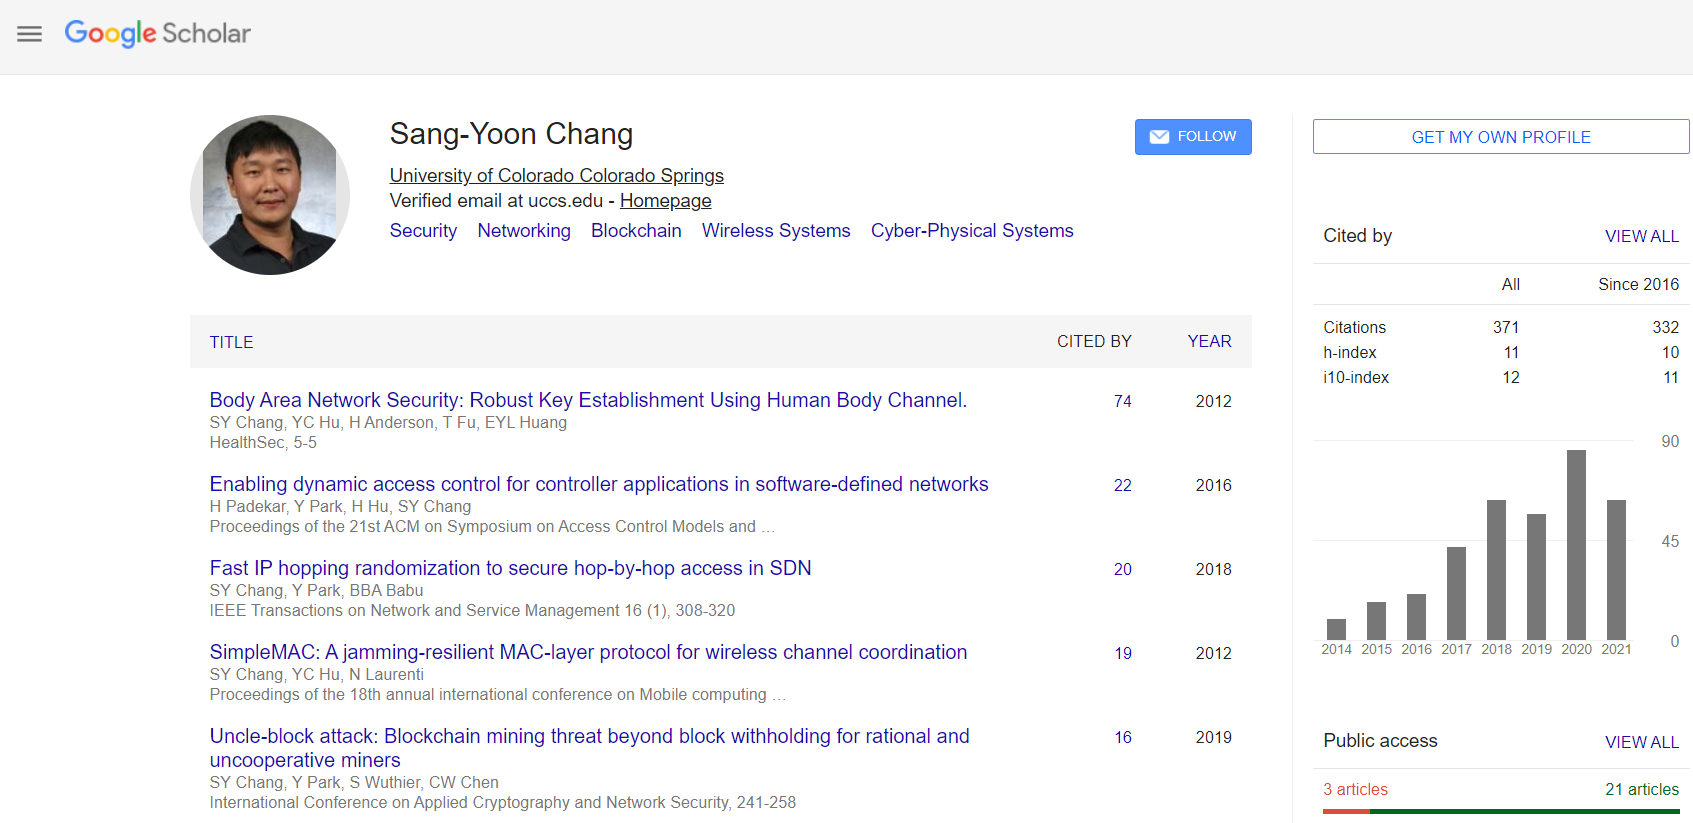
\includegraphics[scale=0.45]{syc1.PNG}
\end{center}

\printbibliography


\end{document}